\documentclass[11pt]{article}
\usepackage{UF_FRED_paper_style}
\usepackage{lipsum}
\onehalfspacing

\setlength{\droptitle}{-5em} %% Don't touch

\title{Tarea1: Juegos en forma extensiva
}

\author{Augusto Rico\\
    \href{mailto:arico@unal.edu.co}{\texttt{arico@unal.edu.co}}}

\date{\today}

\begin{document}

\setstretch{.8} %% Don't touch
\maketitle

% %%%%%%%%%%%%%%%%%%%%%%%%%%%%%%%%%%%%%%%%%%%%%%%%%%%%%%%%%%
% %%%%%%%%%%%%%%%%%%%%%%%%%%%%%%%%%%%%%%%%%%%%%%%%%%%%%%%%%%
% BODY OF THE DOCUMENT
% %%%%%%%%%%%%%%%%%%%%%%%%%%%%%%%%%%%%%%%%%%%%%%%%%%%%%%%%%%
% %%%%%%%%%%%%%%%%%%%%%%%%%%%%%%%%%%%%%%%%%%%%%%%%%%%%%%%%%%

\begin{figure}[h]
    \begin{minipage}[t]{0.5\textwidth}
        \vspace{0pt}
        \begin{flushleft}
        se eligió el siguiente juego en forma extensiva para la tarea,
        obtenido del libro Rationality in Extensive Form Games de \citet{Perea_2001}.\\
        El juego podemos resolverlo mediante induccion hacia atras para obtener los equilibrios
        puros, por lo que iniciaremos con $x_4$ donde el jugador $1$ jugara $j$ que es la estrategia
        que maximiza para el jugador $1$, no obstante en ese caso es mejor para el jugador haber jugado en $x_2$
        la estrategia $f$ dado que $2>1$.\\
        \end{flushleft}
    \end{minipage}
    \hfill
    \begin{minipage}[t]{0.5\textwidth}
        \vspace{0pt}
        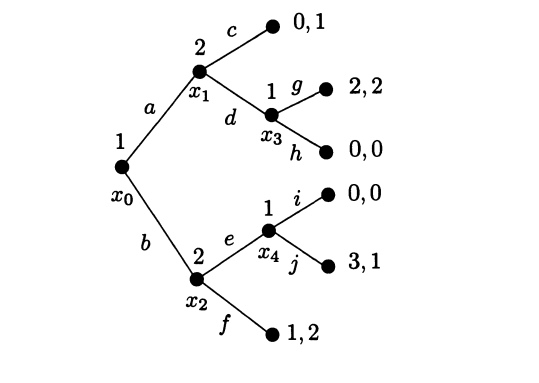
\includegraphics[width=\textwidth]{Screenshot from 2023-05-23 15-21-47.png}
        \label{fig:my_label}
    \end{minipage}
\end{figure}

\begin{flushleft}
    si ahora hacemos induccion hacia atras iniciando en el nodo $x_3$ vemos que para el jugador $1$ la mejor
    estrategia va a ser jugar $g$, estrategia que tambien sera la preferia por el jugador $2$, por lo que este jugador va a preferir la estrategia $g$\\
    con esto sabemos entonces que el equilibrio puro va a estar caracterizado por las estrategias $((a,g),(f,d))$.
\end{flushleft}

\bibliography{references.bib} 


\end{document}